\chapter{Introdução}
Num mundo altamente mecanizado, a força e o torque dentro de todas as grandezas, são as mais comuns. Estas têm um papel significativo nos aparelhos de medição de massa e células de carga usadas na indústria e retalho, nos automóveis e nas aeronaves, no aperto de tampas de frascos de medicina e parafusos.\cite{book-9}
\\
\\
A massa é uma das grandezas fundamentais, uma propriedade intrínseca de um objeto, que se mede pela sua resistência à aceleração.\cite{book-2}
%melhorar imagen
\begin{figure}[H]
	\centering
	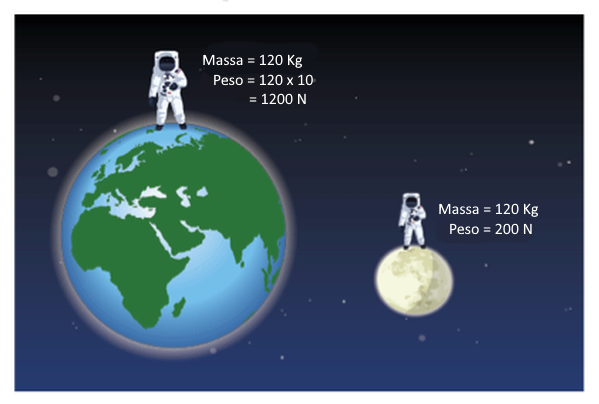
\includegraphics[width=\linewidth]{./image/PESTA/fisica/mass-1.png}
	\caption{Peso e Massa}
	\label{mass}
\end{figure}
Através da medição do peso, isto é, da força gravitacional exercida num dado objeto, podemos calcular a massa. \cite{book-2}
\\
\\
A massa dos objetos pode ser medida por balanças utilizando vários métodos, tais como as alavancas convencionais, por  molas e sistemas mais modernos, tais como, balanças digitais.
\\
\\
As balanças digitais estão presentes no nosso dia a dia, e tornaram-se numa ferramenta indispensável na indústria, comércio e laboratórios. Determinar a massa dos objetos facilitou a moeda de troca no comércio, e tornou-se num pilar fundamental da física e seu desenvolvimentos. Existe uma demanda, tanto na área comercial como na industrial, que empurra o desenvolvimento dos sensores para obter melhores resultados quanto a precisão e imunidade de influências exteriores na medição das grandezas mencionadas.\\
\\
A importância desta grandeza (massa), foi o mote para o projeto proposto: a implementação de uma balança digital para uso doméstico, usando os meios que estão disponíveis no mercado.
\section{Objetivos}
O objetivo principal deste projeto será a implementação de uma balança digital economicamente viável, usando os sensores e equipamentos disponíveis no mercado, para ter um produto útil e fácil de ser replicado.
\\
\\
Escolher o sensor adequado e meios de tratamento da informação e comunicação, será o objeto de estudo. Tendo como foco a utilização de um \textit{Embeded System} utilizando as ferramentas necessárias para o executar.
\\
\\
No final o produto obtido será testado, de forma a tentar aperfeiçoar, fazer melhorias, alterações e adaptações que possam surgir, de forma a simplificar o projeto e torná-lo mais atraente ao consumidor final.
\section{Calendarização}
O segundo semestre teve inicio em 8 de Março, num ambiente de pandemia COVID-19 período durante o qual fomos forçados ao ensino à distancia, e todo o trabalho teve de ser acompanhado \textit{online} pelos docentes. No entanto foi necessário organizar as tarefas pretendidas de acordo com o plano abaixo descrito, para poder fazer a entrega deste trabalho antes da data limite da época normal (28 de Junho de 2021).
%%%%%%%%%%%%%%%%%%%%%%%%%%%%%%%%%%%%%%%%%%%%%%%%%%%%%%%%%%
\begin{table}[H]
	\caption{Calendarização das tarefas}
	%\begin{sidewaysfigure}
	\begin{ganttchart}[vgrid, hgrid]{1}{20}
		\gantttitle{Março}{5} 
		\gantttitle{Abril}{5}
		\gantttitle{Maio}{5}
		\gantttitle{Juno}{5}\\
		\gantttitlelist{1,...,20}{1}\\
		%First Group
		\ganttgroup{Requisitos}{2}{10} \\
		\ganttbar{Material}{3}{5} \\
		\ganttbar{\textit{Template} LaTeX}{5}{10} \\
		\ganttbar{\textbf{IDE} \textit{Template}}{3}{10}\\
		%\ganttlink{elem0}{elem1}
		%\ganttlink{elem1}{elem2}
		%\ganttlink{elem2}{elem3}
		%\ganttmilestone{Milestone 1}{11}
		%Second Group
		\ganttgroup{Projecto}{3}{20} \\
		\ganttbar{Kit Desenvolvimento}{3}{4} \\
		\ganttbar{Montagen Mesa Sensor}{5}{7} \\%5 7
		\ganttbar{HX711 comunicação}{4}{10} \\%4 8
		\ganttbar{Programação e ensaio}{4}{20}\\
		%\ganttlink{elem4}{elem5}
		%\ganttlink{elem5}{elem6}
		%\ganttlink{elem6}{elem7}
		%\ganttmilestone{Milestone 1}{11}
		%Third Group
		\ganttgroup{Relatório}{9}{20} \\
		\ganttbar{Literatura}{8}{12} \\
		\ganttbar{Análise documentação}{9}{12} \\
		%\ganttbar{Validação}{10}{12} \\
		\ganttbar{Execução}{10}{20}
		%\ganttlink{elem8}{elem9}
		%\ganttlink{elem9}{elem10}
		%\ganttlink{elem10}{elem11}
		%\ganttmilestone{Milestone 1}{11}
	\end{ganttchart}
	\label{gantt}
%\end{sidewaysfigure}
\end{table}
\section{Organização do Relatório}
No capítulo 1 é feita uma contextualização do trabalho realizado e do seu propósito face às necessidades do mundo atual.
\\
\\
No capítulo 2 é apresentada uma breve história da evolução das balanças, e depois um estudo da balança digital.
\\
\\
No capitulo 3 é apresentado a balança digital, seus componentes e características descrevendo seus funcionamentos.
\\
\\
No capitulo 4 é descrito o software utilizado, estrutura do programa, e a implementação do código.
\\
\\
O capitulo 5 é a validação do projeto  e seu funcionamento.
\\
\\
O capitulo 6 são exposto as conclusões e futuras possíveis alterações de melhoramento do produto.
%%%%%%%%%%%%%%%%%%%%%%%%%%%%%%%%%%%%%%%%%%%%%%%%%%%%%%%%%%
\chapter{Evolução da balança}
%%%%%%%%%%%%%%%%%%%%%%%%%%%%%%%%%%%%%%%%%%%%%%%%%%%%%%%%%%
\section{O aparecimento e a evolução da balança}
As balanças foram criadas por necessidade durante o desenvolvimento do comércio na antiguidade. Os produtos que não recorriam a contagem por unidades, tais como objetos irregulares (por exemplo o ouro) tinha de se quantificar o seu valor, e a forma de medir a sua massa tornou-se numa variável de medição para a troca de bens.
\\
\\
A relíquia mais antiga de uma balança de medir massa foi descoberta na vila de \textit{Indus River}, perto da região hoje conhecida como Paquistão, e estima-se ser por volta de 2000 A.C.
\\
Estas primeiras balanças eram alavancas em equilíbrio. $[ \; F_{1} \times b_{1c} = F_{2} \times b_{2c} \; ]$. Nos extremos eram colocados cestos estando este conjunto centrado no seu centro de massa. Assim, se os pesos colocados nos dois cestos fossem iguais, a alavanca ficava em equilíbrio (na horizontal). Esse tipo de balança era um sistema de comparação, com recurso a pesos fixos estabelecidos como norma e designados de \textbf{contra-pesos}.
\\
\begin{minipage}[!b]{0.45\linewidth}
	\begin{figure}[H]
		\centering
		\includegraphics[height=7cm]{./image/PESTA/general/balanca_1.jpg}
		\caption{Balança medieval}
		\label{balanca_1}
	\end{figure}
\end{minipage}
\hspace{2.2cm}
\begin{minipage}[!b]{0.45\linewidth}
	\begin{figure}[H]
		\centering
		\includegraphics[height=7cm]{./image/PESTA/general/balanca_4.jpg}
		\caption{Balança de laboratório}
		%\caption{Balança moderna \cite{book-7}}
		\label{balanca_4}
	\end{figure}
\end{minipage}
\newline
\newline
\newline
Este sistema tem grande precisão, mas também pode se facilmente adulterar.
\\
\\
\\
Os métodos de medir a massa de objetos não conheceram nenhumas melhorias tecnológicas relevantes até à era industrial. Só nos fins do século \textit{XVIII} é que o meio de medir a massa de objetos não dependia de \textbf{contra-pesos}. As balanças por molas foram inventados por volta de 1770 em Inglaterra por \textit{Richard Salter}, um fabricante de balanças.
\\
\begin{figure}[H]
	\centering
	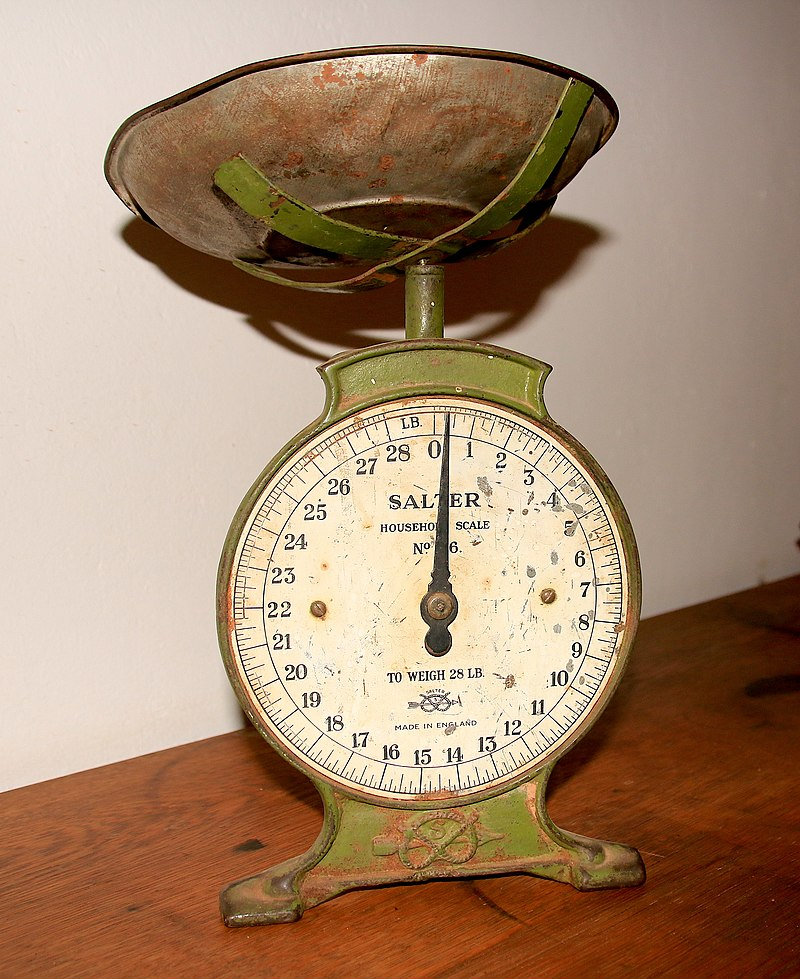
\includegraphics[scale=.3]{./image/PESTA/general/Weigh_Scale_Salter_1.jpg}
	\caption{Balança de Salter}
	\url{https://en.wikipedia.org/wiki/Salter_Housewares}
	\label{Weigh_Scale_Salter_1}
\end{figure}
A balança por mola, como o nome implica, mede a pressão (ou sua tensão) exercida sobre a mola para determinar a massa do objeto. Este tipo de balanças ainda é muito comum nos dias de hoje, por serem bastante económicas de fabricar, mas não têm tanta precisão como as eletrónicas desenvolvidas e aperfeiçoadas durante o século \textit{XX}.
\begin{minipage}[!b]{\linewidth}
	\begin{figure}[H]
		\captionsetup{justification=raggedright,singlelinecheck=false}
		\flushleft
		\includegraphics[height=7cm]{./image/PESTA/general/Public_Body_Scales_1.jpg}
		\hspace{.8cm}
		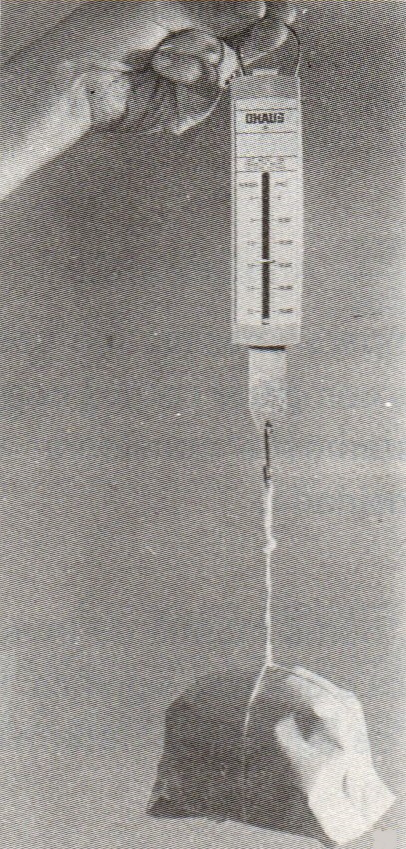
\includegraphics[height=7cm]{./image/PESTA/general/Balanca_Mola_1.jpg}
		\caption{Balanças de Mola}
		\label{Balanca_Mola_1}
	\end{figure}
\end{minipage}
\minipagespace{.3}
\section{A balança eletrónica}
%Desenvolver mais
As balanças eletrónicas mais modernas, utilizam resistências elétricas instaladas sobre materiais flexíveis por onde passa uma corrente elétrica, onde é possível detetar a variação de condutividade das resistências. Esta variação é proporcional à pressão exercida sobre esse material, trata-se dos sensores \textit{strain gauge}. As células de carga são materiais desenhados com uma estrutura para ter o mesmo comportamento de uma mola, dando-lhe uma caraterística de proporcionalidade entre a pressão exercida e o deslocamento provocado no material onde estão colocados os sensores (\textit{strain gauge}) que detetam essa tensão mecânica e compressão. As células de carga são os sensores mais comuns usadas nas balanças digitais, porque geram um sinal proporcional a força ou pressão. De notar que existe muitos tipos de células de carga para diferentes gamas de massas, porque todas as molas tem um ponto de rotura da sua elasticidade onde perde sua caracteristica de ser uma mola.
\\
\begin{figure}[H]
	\centering
	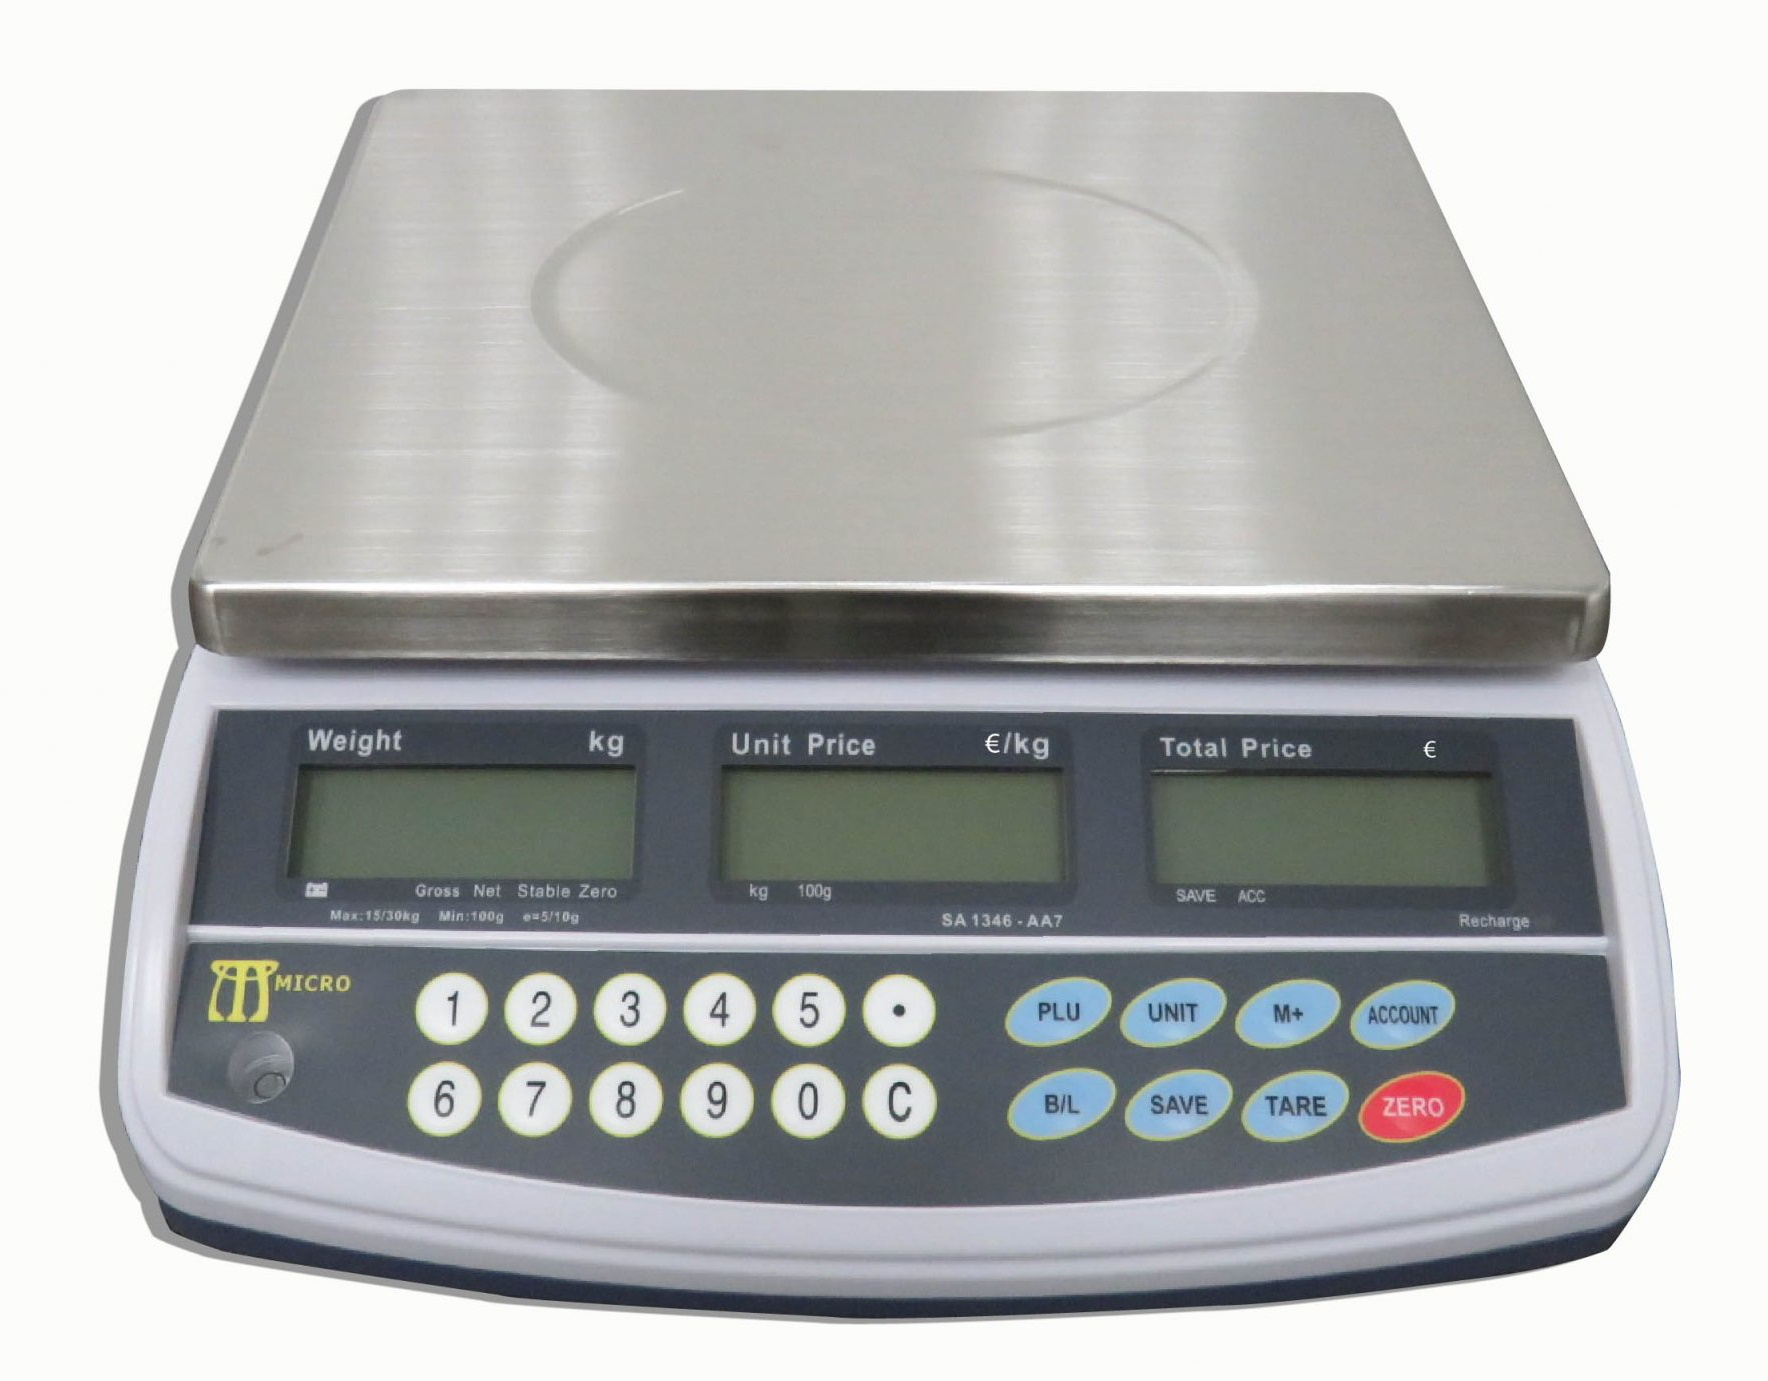
\includegraphics[height=7cm]{./image/PESTA/general/Scale_1.jpg}
	\caption{Balança eletrónica}
	\label{Scale_1}
\end{figure}
No projeto proposto será utilizada uma \textbf{célula de carga}, que segue o princípio acima mencionado. Estas células têm sensores \textit{\textbf{strain gauges}} ligadas em ponte de \textit{Wheatstone}, que vão detetar a distorção (pressão) do material, ou seja, da célula de carga e gerar um sinal de diferença de potencial proporcional à força exercida. Seque o mesmo princípio de uma mola. Todas as molas tem uma constante de elasticidade conhecida pela lei de Hooke \cite{book-3} \textit{equação} \ref{eq:Hooke}.\\
%\\
%As expressões aparecem sem ligação ao texto
%Deve desenvolver mais esta parte, resultando numa mais elaborada fundamentação teórica
\begin{equation}
	\label{eq:Hooke}
	K = \frac{\Delta x}{F}
\end{equation}
\equationspace{.5}
Na \textit{figura} \ref{Hooke-1} temos um exemplo prático.
\begin{figure}[H]
	\centering
	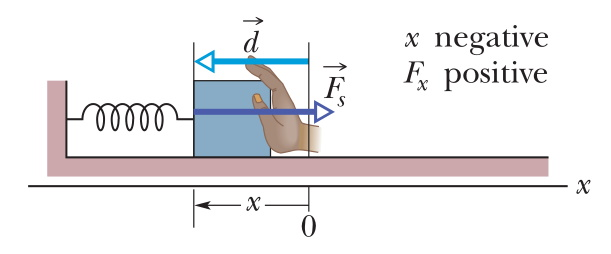
\includegraphics[height=5cm]{./image/PESTA/fisica/Hooke-1.jpg}
	\caption{Exemplo lei de Hooke \cite{book-3}}
	\label{Hooke-1}
\end{figure}
Em que.
\begin{equation}
	\label{eq:Lei-de-Hooke}
	F_x = -K \; x
\end{equation}
E a energia dissipada pela mola é determinada pela expressão \ref{eq:Hooke-Energia}
\begin{equation}
	\label{eq:Hooke-Energia}
	W_s = - \; \frac{1}{2} \; K x^2
\end{equation}
Outros tipos de células de carga, tais como as pneumáticas e hidráulicas, convertem a pressão num sinal elétrico, que é proporcional à força nela exercida, de acordo com a expressão \ref{eq:Preasure}.
\begin{equation}
	\label{eq:Preasure}
	P = \frac{F}{A}
\end{equation}
As células de carga capacitivas são outro exemplo de como obter um sinal proporcional da força imposta como carga. Neste caso, é medida a sua capacidade de acordo com o afastamento ou aproximação das placas dos elétrodos, expressão \ref{eq:Capacity}.
\begin{equation}
	\label{eq:Capacity}
	C = \varepsilon_{0} \; \varepsilon_{r} \; \frac{A}{d}
\end{equation}
Também existem células, que utilizam o princípio de ressonância, desfasamento de fase, e pelo efeito \textit{Doppler} para determinar a pressão ou distorção das células de carga em que resulta numa medição.
\\
\\
Pode-se dizer que, em todos os casos se determina a força resultante através do deslocamento no espaço.
\\
\\
Como se pode observar existe diversos tipos de células de carga, é a peça principal que mede informação analógica da vida real para outra analógica de sinal elétrico, uma etapa de conversão onde podemos utilizar nos nossos sistemas eletrónicos para determinar seu valor.
\\
É nesta etapa em que precisamos de outra conversão, de um sinal analógico elétrico para outro que seja do tipo discreto para poder ser tratado digitalmente, estou a falar dos \ac{adc}, e como a maioria dos sensores geram sinais com magnitude muito pequenas é frequente necessitar também de uma pré amplificação com uma filtragem de ruídos.
\\
Depois de chegar ao mundo digital, já trabalhamos com \textit{bit}, \textit{nibble} e \textit{bytes}. A partir daqui entramos no mundo da programação, onde a informação pode ser manipulada de forma a cumprir os objetivos que se pretende, e que neste caso também vai ser objeto de estudo.
É nesta etapa que se tem de determinar que tipo de balança digital pretendemos e suas caraterísticas, pois pode-se implementar das mais simples até as mais complexas.
%%%%%%%%%%%%%%%%%%%%%%%%%%%%%%%%%%%%%%%%%%%%%%%%%%%%%%%%%%
\begin{comment}
Measurement devices need to be robust to withstand changing environmental influences such as temperature, vibration, and humidity, and they must also provide reliable measurement over long periods of time. Mechanical interfacing of the devices can be difficult and can influence final measurement. The forces and torques may change rapidly, and so the devices must have adequate frequency and transient responses.\\
There are several methods to measure forces and torques. Often, the force to be measured is converted into a change in length of a spring element. The change in dimensions is subsequently measured by a sensor, for example, a piezoresistive, a capacitive or a resonant sensor.\\
It is not so surprising, therefore, that most force and torque measurement devices utilize the long and well-established resistance strain gauge technology.\\
Unfortunately, the metallic resistance strain gauge is relatively insensitive such that in use it is normal to obtain only several millivolts of analog voltage before amplification, and the gauges must not be significantly overstrained. The rangeability and overloading capabilities are seriously restricted. Also, the gauges consume relatively high electrical power (e.g., 250 mW).\\
In general, measurement instrumentation now needs smaller sensing devices of lower power consumption and with greater rangeability and overload capabilities.\\
Greater compatibility with digital microelectronics is highly desirable. Noncontact and wireless operation is sometimes needed, and in some cases batteryless devices are desirable. Production of measurement devices using metallic resistance strain gauges can be relatively labor intensive and skilled, and may require relatively ineffi-cient calibration procedures.\\
In recent years some instrument manufacturers of force and torque measure-ment devices have moved away from using resistance strain gauges. Already, one leading manufacturer of weighing machines for retail and industrial applications now uses metallic and quartz resonant tuning fork technologies, and smaller compa-nies have established niche markets using surface acoustic wave (SAW) technology, optical technology, and magnetoelastic technology.\\
Further commercial developments are taking place to enhance device manufacturability and improve device sensitivity and robustness in operation. Measurement on stiffer structures at much lower strain levels is now possible. The worldwide sensor research base is very active in exploring MEMS for sensing force and torque, and the rest of this chapter will review the current situation and future prospects.\\
\\
The market pull provided by the automotive industry—for example, for manifold air pressure sensors has led to the development of successful devices and technologies that have benefited a wide range of other pressure sensing applications.
\end{comment}
